\documentclass[a4paper, 12pt]{article}
% ABNT
\usepackage[lmargin=3cm, tmargin=3cm, rmargin=2cm, bmargin=2cm]{geometry}
\usepackage[onehalfspacing]{setspace} % Espaçamento de 1,5
\usepackage[T1]{fontenc}
\usepackage[brazil]{babel} % Traduzir para PT-BR
\usepackage{multirow}
% Pacotes essenciais
\usepackage[utf8]{inputenc} % Permite utilizar caracteres especiais: Ex: ç á à...
\usepackage{amsmath, amsfonts, amssymb}
\usepackage{float}
\usepackage{graphicx} % p/ add gráficos
\usepackage{IEEEtrantools} % Para fazer boas equações
% Introduzindo comandos utilizados
\usepackage{pgffor} % Pacote para laço condicional
\usepackage{textgreek}

% Comando para iniciar o cabeçao
\newcommand{\initcab}[2]{

\begin{tabular}{lllll}
	\multirow{4}*{
\includegraphics[width=50px]{figs/logo_ufc.png}}    &			\multicolumn{4}{l}{\Large{\textbf{Universidade Federal do Ceará}}} \\
																	&			Disciplina:&\multicolumn{2}{l}{Processamento Estatístico de Sinais}\\
																	&			Professor:&Charles Casimiro Cavalcante \\
																	&			Estudante:&Rubem Vasceconcelos Pacelli & Matrícula: 474725 &
\end{tabular}

\begin{flushright}
\footnotesize{#1 de 2019}
\end{flushright}

{\Large Lista #2}

}

% Comando para a craiação de Rx
\newcommand{\RxTres}{
\begin{bmatrix}
 R_{dx}(0)  & R_{dx}(1)  & R_{dx}(2)\\
 R_{dx}(-1) & R_{dx}(0)  & R_{dx}(1)\\
 R_{dx}(-2) & R_{dx}(-1) & R_{dx}(0)\\
\end{bmatrix}
}

\newcommand{\RxTresE}{
\begin{bmatrix}
 \textEpsilon\left[ x^{2}\left[ n\right] \right] & 
 \textEpsilon\left[ x\left[ n\right] x\left[ n-1\right] \right] &
 \textEpsilon\left[ x\left[ n\right] x\left[ n-2\right] \right] \\
 \textEpsilon\left[ x\left[ n-1\right] x\left[ n\right] \right] &
 \textEpsilon\left[ x^{2}\left[ n-1\right] \right] &
 \textEpsilon\left[ x\left[ n-1\right] x\left[ n-2\right] \right] \\
 \textEpsilon\left[ x\left[ n-2\right] x\left[ n\right] \right] &
 \textEpsilon\left[ x\left[ n-2\right] x\left[ n-1\right] \right] &
 \textEpsilon\left[ x^{2}\left[ n-2\right] \right]
\end{bmatrix}
}


\newcommand{\RxDois}{
\begin{bmatrix}
 R_x(0)  & R_x(1)\\
 R_x(-1) & R_x(0)\\
\end{bmatrix}
}

\newcommand{\RxDoisE}{
\begin{bmatrix}
 \textEpsilon\left[ x^{2}\left[ n\right] \right] & 
 \textEpsilon\left[ x\left[ n\right] x\left[ n-1\right] \right] \\
 \textEpsilon\left[ x\left[ n-1\right] x\left[ n\right] \right] &
 \textEpsilon\left[ x^{2}\left[ n-1\right] \right]
\end{bmatrix}
}

\newcommand{\RdxDois}{
\begin{bmatrix}
 R_{dx}(0)\\
 R_{dx}(-1)\\
\end{bmatrix}
}

\newcommand{\RdxDoisE}{
\begin{bmatrix}
 \textEpsilon\left[ x\left[ n\right]d\left[ n\right] \right] &  \\
 \textEpsilon\left[ x\left[ n-1\right] d\left[ n\right] \right]
\end{bmatrix}
}
% Alguns comas de notações
\newcommand{\RxCor}{\mathbf{R_{x}}}
\newcommand{\RdxCor}{\mathbf{R_{\textnormal{d}x}}}
\newcommand{\wCor}{\mathbf{w_o}}
\newcommand{\xCor}{\mathbf{x}}
\newcommand{\LambdaCor}{\mathbf{\Lambda}}
\newcommand{\ModalCor}{\mathbf{Q}}
\newcommand{\EigenVCor}{\mathbf{q}}
\newcommand{\ACor}{\mathbf{A}}
\newcommand{\FLPoe}{\textit{Forward Linear Prediction} (FLP) \textit{one-step}}
\newcommand{\wf}{\mathbf{w_f}}
\newcommand{\Rx}{\mathbf{R_{x}}}
\newcommand{\rxs}{\mathbf{r}_{\mathbf{x},s}}

\begin{document}
\initcab{Novembro}{4}

\begin{enumerate}
	\item \hspace{1cm} % Apenas para começar outra linha
	A Função de correlação do sinal de entrada é
		\begin{IEEEeqnarray}{rCl}
			\RxCor & = & \RxDois \nonumber \\
			& = & \RxDoisE \nonumber \\
			\RxCor & = & \begin{bmatrix}  1 & 0.5 \\ 0.5 & 1 \end{bmatrix}
		\end{IEEEeqnarray}
		A Funçaõ de correlação cruzada entre o sinal de entrada e o sinal desejado é
		\begin{IEEEeqnarray}{rCl}
			\RdxCor & = & \RdxDois \nonumber \\
			& = & \RdxDoisE \nonumber \\
			\RdxCor & = & \begin{bmatrix}  0.5 \\ 0.25 \end{bmatrix}
			\label{Rdx}
		\end{IEEEeqnarray}	
	
	\begin{enumerate}
		% Item A
		\item
		\begin{IEEEeqnarray}{rCl}
			\RxCor^{-1} & = & \frac{1}{det\left(\RxCor\right)}\cdot Adj\left(\RxCor\right) \nonumber \\
			\RxCor^{-1}& = & \begin{bmatrix} 1.33 & -0.67 \\
											 .67  &  1.33 \end{bmatrix}
			\label{Rxinv}
		\end{IEEEeqnarray}
		
		A equação de Wiener–Hopf fornece os coeficientes do filtro ótimo. Para os matrizes dadas nas equações \eqref{Rdx} e \eqref{Rxinv}, os parâmetros do filtro FIR é dado por \cite{SimonHaykin}
		\begin{IEEEeqnarray}{rCl}
			\wCor & = & \RxCor^{-1} \RdxCor \nonumber \\
			\wCor & = & \begin{bmatrix} 0.5\\
							   	  0 \end{bmatrix}
			\label{WienerHopf}
		\end{IEEEeqnarray}
		% Item B
		\item
		Seja $\sigma^2_d$ a variância do sinal desejado, o mínimo erro médio quadrático fornecido pelo filtro de Wiener é \cite{SimonHaykin}
		\begin{IEEEeqnarray}{rCl}
			J_{min} & = & \sigma^2_d -\RdxCor^H\wCor \nonumber \\
			J_{min} & = & \sigma^2_d -0.25
			\label{Jmin}
		\end{IEEEeqnarray}
		% Item C
		\item
		Uma expressão importante obtida a partir do filtro de Wiener é o valor da função de custo em torno do ponto ótimo, que pode ser expressada em termos dos autovalores e autovetores da matriz $\RxCor$. Considere o sinal de erro da saída de um filtro de FIR cujos os coeficiente não minimizam a função custo (i.e., filtro não-ótimo, $\mathbf{w}\ne\wCor$), o erro quadrático é
		\begin{IEEEeqnarray}{rCl}
			|e\left[n\right]|^2 & = & \left( d\left[n\right] - \mathbf{w}^H\mathbf{x} 					\right)\left( d\left[n\right] - \mathbf{w}^H\mathbf{x} \right)^H \nonumber \\
			 & = & \left( d\left[n\right] - \mathbf{w}^H\mathbf{x} \right)\left( d\left[n					\right] - \mathbf{x}^H\mathbf{w} \right)  \nonumber \\
			  & = & |d\left[n\right]|^2 - d\left[n\right]\mathbf{x}^H\mathbf{w}
			  - d\left[n\right]\mathbf{w}^H\mathbf{x} + \mathbf{w}^H\mathbf{x}\mathbf{x}^H				\mathbf{w}
			\label{erro}  
		\end{IEEEeqnarray}
		Calculando a média na equação \eqref{erro} e observando que $\mathbf{w}^H\mathbf{x}=\mathbf{x}^H	\mathbf{w}$, têm-se:
		\begin{IEEEeqnarray}{rCl}
			J\left(\mathbf{w}\right) & \triangleq & E\left[|e\left[n\right]|^2\right]  \nonumber \\
			 & = & E\left[ |d\left[n\right]|^2 - d\left[n\right]\mathbf{x}^H\mathbf{w}
			  - d\left[n\right]\mathbf{w}^H\mathbf{x} + \mathbf{w}^H\mathbf{x}\mathbf{x}^H				\mathbf{w} \right]  \nonumber \\
			   & = & \sigma^2_d - 2\mathbf{w}^H\RdxCor + \mathbf{w}^H\RxCor\mathbf{w}
			   \label{Jw}
		\end{IEEEeqnarray}
		Observe que se substituirmos \eqref{WienerHopf} em \eqref{Jw}, obteremos a equação \eqref{Jmin}, ou seja, $J_{min}=J\left(\wCor\right)$. Pode-se analisar como a função custo se comporta em torno do ponto ótimo fazendo com que $\mathbf{w}=\wCor+\Delta\mathbf{w}$, então
		\begin{IEEEeqnarray}{rCl}
			J\left(\wCor+\Delta\mathbf{w}\right) & = & \sigma^2_d - 2\mathbf{\left(\wCor+\Delta\mathbf{w}\right)}^H\RdxCor + \mathbf{\left(\wCor+\Delta\mathbf{w}\right)}^H\RxCor\mathbf{\left(\wCor+\Delta\mathbf{w}\right)}  \nonumber \\
			 & = & J_{min}+\Delta\mathbf{w}^H\RxCor\Delta\mathbf{w}
			   \label{JwDeltaw}
		\end{IEEEeqnarray}
		A matriz $\RxCor$ pode ser diagonalizada em termos da matriz modal (i.e., a matriz formada pelos autovetores) e a matriz diagonal dos autovalores \cite{MouradBarkat}.
		\begin{IEEEeqnarray}{rCl}
			\RxCor & = & \ModalCor^H \LambdaCor \ModalCor
			\label{Diagonalizacao}
		\end{IEEEeqnarray}
		Em que $\ModalCor$ é a matriz modal
		
		\begin{IEEEeqnarray}{rCl}
			\ModalCor & = & \begin{bmatrix} \EigenVCor_1 & \EigenVCor_2 \end{bmatrix} \nonumber \\
			\ModalCor & = & \begin{bmatrix} -0.7071 & 0.7071 \\
			 					   0.7071  & 0.7071\end{bmatrix}
			\label{Modal}
		\end{IEEEeqnarray}

		E $\LambdaCor$ é matriz diagonal formada pelos autovalores \cite{MouradBarkat}		
		\begin{IEEEeqnarray}{rCl}
			\LambdaCor & = & \begin{bmatrix} \lambda_1 & 0 \\
											0 & \lambda_2 \end{bmatrix} \\
			\LambdaCor & = & \begin{bmatrix} 0.5 & 0 \\
											0   & 1.5 \end{bmatrix}
			\label{Lambda}					
		\end{IEEEeqnarray}
		
		Substituindo \eqref{Diagonalizacao} em \eqref{JwDeltaw}, temos:
		\begin{IEEEeqnarray}{rCl}
			J\left(\wCor+\Delta\mathbf{w}\right) & = & J_{min}+\Delta\mathbf{w}^H\ModalCor \LambdaCor \ModalCor^H\Delta\mathbf{w} \\
			& = & J_{min}+\mathbf{v}^H \LambdaCor \mathbf{v}
		\end{IEEEeqnarray}
		
		Em que $\mathbf{v}=\ModalCor^H\Delta\mathbf{w}$.
	\end{enumerate}
	\item 
		Considere a seguinte representação matricial da equação de Wiener–Hopf e da equação da função de custo mínima (mostradas em \eqref{WienerHopf} e \eqref{Jmin}, respectivamente):
		\begin{IEEEeqnarray}{rCl}
			\begin{bmatrix}
				\sigma^2_d & \RdxCor^H \\
				\RdxCor    & \RxCor
			\end{bmatrix}
			\begin{bmatrix}
				1 \\ -\wCor
			\end{bmatrix}
			& = &
			\begin{bmatrix}
				J_{min} \\ \mathbf{0}
			\end{bmatrix} \nonumber \\
			\ACor
			\begin{bmatrix}
				1 \\ -\wCor
			\end{bmatrix}
			& = &
			\begin{bmatrix}
				J_{min} \\ \mathbf{0}
			\end{bmatrix}
			\label{AugmentedWienerHopf}
		\end{IEEEeqnarray}
		
		Em que $\mathbf{0}$ é o vetor nulo com dimensão igual a ordem do filtro de Wiener–Hopf. Com base na equação \eqref{AugmentedWienerHopf}, pode-se facilmente concluir que $\ACor$ é matriz de correlação do vetor aumentado
	\begin{IEEEeqnarray}{c}
		\begin{bmatrix}
				d[n] \\
				\mathbf{x}
		\end{bmatrix}
		\label{VectorAugmented}
	\end{IEEEeqnarray}
	
	Nesta análise, estamos supondo que $d[n]$ possui média nula e, portanto, o segundo momento central é igual ao seu segundo momento, i.e., $\sigma^2_d \triangleq E\left[\left(d[n] - E\left[d[n]\right]\right)^2\right]=E\left[d^2[n]\right]$.
	
	\item % Questão 3
	A Figura \ref{Q2} mostra um diagrama de blocos de uma arquitetura típica de cancelamento de ruído. 
	\begin{figure}[H]
		\centering
		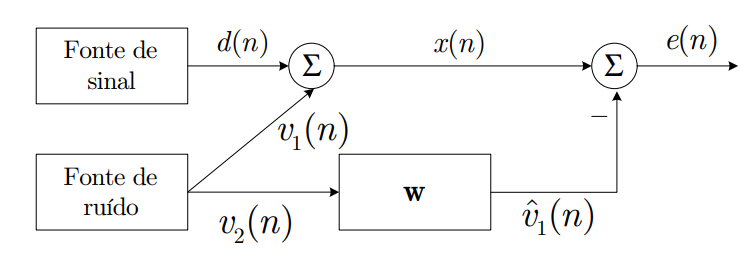
\includegraphics[scale=.45]{figs/Q2.png}
		\caption{Cancelamento de ruído}
		\label{Q2}
	\end{figure}
	
	Cancelamento de ruído é um assunto clássico em sistemas de comunicações no qual se pode utilzar técnicas de processamento estatístico de sinais para estimar o ruído incidente no sinal transmitido e, por fim, suprimi-lo \cite{Proakis}.
	
	Neste tipo de problema, é utilizado dois sensores. Enquanto o primeiro capta o sinal transmitido corrompido pelo ruído (representado na Figura \ref{Q2} como $x[n]$), o segundo sensor capta apenas o ruído do canal (representado como $v_2[n]$). Portanto, os sinais conhecidos para este problema são $v_2[n]$ e $x[n]$.
	
	No entanto, a subtração direta do sinal $v_2[n]$ no sinal recebido não fornece o desempenho desejado, pois, apesar de se originarem da mesma fonte, o ruído captado pelo segundo sensor ($v_2[n]$) é um processo estocástico diferente do ruído que é captado pelo primeiro sensor ($v_1[n]$). Apesar de ambos guardarem uma certa correlação, seus valores para o mesmo instante de amostragem se diferem. Afinal, tratam-se de processos estocásticos, e não determinísticos.
	
	O problema então é: Com base no ruído do segundo sensor ($v_2[n]$), estimar, através da implementação de um filtro de Wiener, a estimativa do ruído que distorce o sinal desejado ($\hat{v}_1[n]$) \cite{Proakis}, \cite{SilvioAbrantes}.
	
	O objetivo do filtro de Wiener é selecionar os coeficiente do filtro FIR de tal forma de minimize a função custo, ou seja:
	\begin{IEEEeqnarray}{rCl}
		\dfrac{\partial}{\partial\mathbf{w}}E\left\{ e[n]e^*[n] \right\} & = & 0\nonumber \\
		E\left\{e[n]\dfrac{\partial e^*[n]}{\partial\mathbf{w}} \right\} & = & 0\nonumber \\
		E\left\{e[n]\dfrac{\partial \left(x^*[n] - \hat{v}_1^*[n]\right)}{\partial\mathbf{w}} \right\} & = & 0\nonumber \\
		E\left\{e[n]\dfrac{\partial \left(x^*[n] - \mathbf{w}^T \mathbf{v_2^*} \right)}{\partial\mathbf{w}} \right\} & = & 0\nonumber \\
		E\left\{e[n]\mathbf{v_2^*}\right\} & = & \mathbf{0}
	\end{IEEEeqnarray}

	Em que $\mathbf{v_2} = \begin{bmatrix} v_2[n] & v_2[n-1] & \cdots & v_2[n-M+1] \end{bmatrix}^T$, $M$ é a ordem do filtro de Wiener e $\mathbf{0}$ é vetor nulo de ordem M. Portanto:
	\begin{IEEEeqnarray}{rCll}
		E\left\{e[n]v_2^*[n-k] \right\} & = & 0 & \textrm{ para } 0 \leq k \leq M-1
	\end{IEEEeqnarray}
	
	Essa equação fornece que, quando o filtro é ótimo, o erro é ortogonal ao sinal de entrada. Substituindo o sinal de erro, têm-se:
	\begin{IEEEeqnarray}{rCl}
		E\left\{\left(x[n]-\hat{v_1}[n]\right) v_2^*[n-k] \right\} & = & 0 \nonumber \\
		E\left\{\left(x[n]- \sum_{i=1}^{M-1}w[i]v_2[n-i] \right) v_2^*[n-k] \right\} & = & 0 \nonumber \\
		E\left\{x[n]v_2^*[n-k]- \sum_{i=1}^{M-1}w[i]v_2[n-i]v_2^*[n-k] \right\} & = & 0 \nonumber \\
		E\left\{x[n]v_2^*[n-k]\right\}- \sum_{i=1}^{M-1}w[i]E\left\{v_2[n-i]v_2^*[n-k] \right\} & = & 0
	\end{IEEEeqnarray}
	
	Com base na Figura \ref{Q2}, pode-se ainda deixar o sinal recebido($x[n]$) em termos do ruído e do sinal transmitido:
	\begin{IEEEeqnarray}{rCl}
		E\left\{(d[n]+v_1)v_2^*[n-k]\right\} & = & \sum_{i=1}^{M-1}w[i]E\left\{v_2[n-i]v_2^*[n-k] \right\} \nonumber \\
		E\left\{d[n]v_2^*[n-k]\right\}+E\left\{v_1[n]v_2^*[n-k]\right\} & = & \sum_{i=1}^{M-1}w[i]E\left\{v_2[n-i]v_2^*[n-k] \right\} \nonumber \\
		R_{d,v_2}[k]+R_{v_1,v_2}[k] & = & \sum_{i=1}^{M-1}w[i]R_{v_2,v_2}[k-i]
		\label{v1&v2}
	\end{IEEEeqnarray}
	
	Observe que o sinal desejado, $d[n]$ e o ruído do segundo sensor, $v_2[n]$, são descorrelacionados, portanto
	\begin{IEEEeqnarray}{rCl}
	R_{d,v_2}[k]=0, \forall k \in \mathbb{Z}
	\label{dv2=0}
	\end{IEEEeqnarray}
		
	Por outro lado, os processos estocásticos $v_1[n]$ e $v_2[n]$ guardam algum tipo de correlação, pois ambos  se originam da mesma fonte. A expressão analítica da função de correlação cruzada que estes dois sinais possuem varia para cada aplicação. A função de autocorrelação de $v_2[n]$ seria, no caso mais descorrelacionado possível, AWGN (do inglês, \textit{Additive white Gaussian noise}), i.e., suas amostras teriam correlação nula em diferenças de instantes diferentes de zero. É importante ressaltar que estamos a considerar que os processos aleatórios envolvidos neste problema são WSS (\textit{Wide Sense Stationary}) e, portanto, considerar-se apenas a diferença entre as amostras uma vez que o deslocamento temporal das mesmas não afeta a função de autocorrelação.
	
	No entanto, o não é possível calcular $R_{v_1,v_2}[k]$ uma vez que o sinal $v_1[n]$ não é conhecido. Felizmente, é fácil mostrar que
	\begin{IEEEeqnarray}{rCl}
		R_{v_1,v_2}[k] & = & E\left\{v_1[n-i]v_2^*[n-k] \right\} \nonumber \\
		R_{v_1,v_2}[k] & = & E\left\{(x[n]-d[n])v_2^*[n-k] \right\} \nonumber \\
		R_{v_1,v_2}[k] & = & E\left\{x[n]v_2^*[n-k]\right\} - E\left\{d[n]v_2^*[n-k]\right\} \nonumber \\
		R_{v_1,v_2}[k] & = & R_{x,v_2}[k] - R_{d,v_2}[k] \nonumber \\
		R_{v_1,v_2}[k] & = & R_{x,v_2}[k]
		\label{v1v2Toxv2}
	\end{IEEEeqnarray}
	
	Substituindo \eqref{dv2=0} e \eqref{v1v2Toxv2} em \eqref{v1&v2}, têm-se:
	\begin{IEEEeqnarray}{rCl}
		\sum_{i=1}^{M-1}w[i]R_{v_2,v_2}[k-i] & = & R_{x,v_2}[k]
	\end{IEEEeqnarray}
	
	Ou, em notação matricial:
	\begin{IEEEeqnarray}{rCl}
		\mathbf{R_{v_2,v_2}w}  & = & \mathbf{R_{x,v_2}} \nonumber \\
		\mathbf{w}  & = & \mathbf{R_{v_2,v_2}^{-1}R_{x,v_2}}
		\label{wiener-q2}	
	\end{IEEEeqnarray}

	Considera-se que $\mathbf{R_{v_2,v_2}}$ possua inversa. O resultado obtido em \eqref{wiener-q2} é exatamente a equação de Wiener–Hopf (ver equação \eqref{WienerHopf}), mas derivado do estudo sobre cancelamento de ruído.
	
	\item % Questão 4
	
		A Figura \ref{FLP} mostra a estutura típica de uma \FLPoe\, \cite{SimonHaykin} \cite{SilvioAbrantes}.
				\begin{figure}[H]
					\centering
					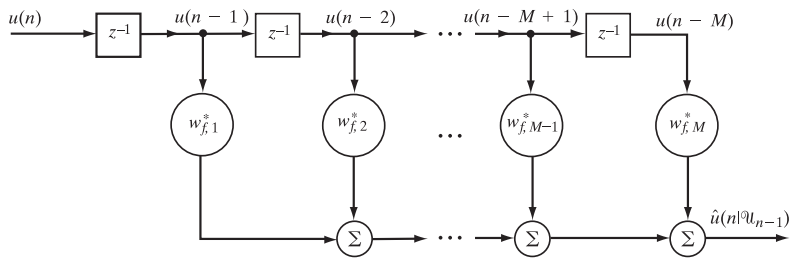
\includegraphics[scale=0.5]{figs/q4.png}
					\caption{\FLPoe.}
					\label{FLP}
				\end{figure}
				
				A otimização do erro quadrático médio também é obtido por meio da implementação do filtro de Wiener. Portanto, todas as equações provenientes do seu estudo são utilizadas na predição linear.
				
				A abordagem clássica fornecida na literatura sobre \FLPoe~é \cite{SimonHaykin}: Dado um vetor de variáveis aleatórias $$\mathbf{u}[n-1] = \begin{bmatrix} u[n-1] & u[n-2] & \cdots & u[n-M+1] \end{bmatrix}^T,$$ predizer o valor da próxima amostra, $u[n]$ (por este motivo que é chamado de \textit{one-step}). 
				
				No entanto, neste problema, o sinal de entada é $x[n]=s[n+a]+s[n-4a]$. Além disso, não se deseja a próxima amostra, mas sim de $d[n]=s[n-a]$. Da equação de Wiener em \eqref{WienerHopf}, temos:
				\begin{IEEEeqnarray}{rCl}
					\wf & = & \Rx^{-1} \rxs
					\label{WienerHopfQ4}
				\end{IEEEeqnarray}
				
				Em que $\Rx$ é a matriz correlação do sinal de entrada, dado por
				\begin{IEEEeqnarray}{rCl}
					\Rx = \begin{bmatrix} R_x(0) & R_x(1) \\
										R_x(-1) & R_x(0) \end{bmatrix}
					\label{RxM}
				\end{IEEEeqnarray}
				
				e $\rxs$ é a matriz de correlação cruzada entre o sinal de entrada e o sinal desejado, ou seja:
				\begin{IEEEeqnarray}{rCl}
					\rxs = \begin{bmatrix} R_{x,s}(0) \\ R_{x,s}(1) \end{bmatrix}
					\label{rxsM}
				\end{IEEEeqnarray}
				
				A função de auto correlação do sinal $x[n]$ é:
				\begin{IEEEeqnarray}{rCl}
					R_x(\tau) & = & E\left[x[n]x[n-\tau] \right] \nonumber \\
					& = & E\left[\left(s[n+a]+s[n-4a]\right) \left(s[n+a-\tau]+s[n-4a-\tau] \right) \right] \nonumber \\
					& = & 2R_s(\tau) + R_s(\tau+5a) + R_s(\tau-5a)
					\label{RxTau}
				\end{IEEEeqnarray}
					
				E a função de correlação cruzada é:
				\begin{IEEEeqnarray}{rCl}
					R_{x,s}(\tau) & = & E\left[x[n]s[n-a-\tau] \right] \nonumber \\
					R_{x,s}(\tau) & = & E\left[\left(s[n+a]+s[n-4a]\right)s[n-\tau-a] \right] \nonumber \\
					R_{x,s}(\tau) & = &  R_s(\tau+2a)+R_s(\tau-3a)
					\label{rxsTau}
				\end{IEEEeqnarray}
		
		Substituindo \eqref{RxM} e \eqref{rxsM} em \eqref{WienerHopfQ4}, têm-se
		\begin{IEEEeqnarray}{rCl}
			\wf & = & \dfrac{1}{\left|\Rx\right|} \begin{bmatrix} R_x(0)R_{x,s}(0)-R_x(1)R_{x,s}(1)\nonumber\\
			 	        		         -R_x(-1)R_{x,s}(0)+R_x(0)R_{x,s}(1)	                
				      \end{bmatrix} \\
			& = & \dfrac{1}{\left|\Rx\right|} \begin{bmatrix}
					\mathbf{w_{f1}}\\ \mathbf{w_{f2}} \end{bmatrix}
		\end{IEEEeqnarray}
		
		Em que
		\begin{IEEEeqnarray}{rCl}
			\mathbf{w_{f1}} & = & \left(R_{s}\left(2\,a\right)+R_{s}\left(-3\,a\right)\right)\,\left(2R_{s}\left(5\,a\right)+2\right) \nonumber \\
			&& \negmedspace {} -\left(R_{s}\left(2\,a+1\right)+R_{s}\left(1-3\,a\right)\right)\,\left(2\,R_{s}\left(1\right)+R_{s}\left(1-5\,a\right)+R_{s}\left(5\,a+1\right)\right) \IEEEeqnarraynumspace
			\label{wf1}
		\end{IEEEeqnarray}
		e
		\begin{IEEEeqnarray}{rCl}
			\mathbf{w_{f2}} & = & \left(R_{s}\left(2\,a+1\right)+R_{s}\left(1-3\,a\right)\right)\,\left(2R_{s}\left(5\,a\right)+2\right) \nonumber\\
			&& \negmedspace {} -\left(R_{s}\left(2\,a\right)+R_{s}\left(-3\,a\right)\right)\,\left(2\,R_{s}\left(-1\right)+R_{s}\left(-5\,a-1\right)+R_{s}\left(5\,a-1\right)\right) \IEEEeqnarraynumspace
			\label{wf2}
		\end{IEEEeqnarray}
		Para essas simplificações, utilizamos as seguintes propriedades de processos aleatórios WSS \cite{LeonGarcia}:
		\begin{itemize}
			\item $R_s(\tau)$ é uma função par, i.e., $R_s(\tau)=R_s(-\tau)$
			\item $R_s(0)=E\left[s^2[n]\right]=VAR\left[s[n]\right]=1$. Lembre-se que $E\left[s[n]\right]=0$.
		\end{itemize}
		
		Infelizmente, não é possível simplificar mais as equações \eqref{wf1} e \eqref{wf2} pois $s[n]$ não é uma sequência de variáveis aleatórias independentes, portanto $E\left[s[n]s[n-\tau]\right]\neq E\left[s[n]\right]E\left[s[n-\tau]\right]$
		
		\item %%%% Questão cinco
			\begin{enumerate}
				\item
					A matriz de correlação do sinal de entrada é dada por
					\begin{IEEEeqnarray}{rCl}
						\Rx = \begin{bmatrix} R_x(0) & R_x(1) \\
									R_x(-1) & R_x(0) \end{bmatrix}
					\end{IEEEeqnarray}
					
					Em que $R_x(0) = 1$ e $R_x(1)=R_x(-1)=0$. Portanto, temos
					\begin{IEEEeqnarray}{rCl}
						\Rx & = & \begin{bmatrix} 1 & 0 \\
									   		     0 & 1 \end{bmatrix}
						\label{q5Rx}
					\end{IEEEeqnarray}
					
					Note que esta matriz de correlação é uma matriz identidade. Logo $\Rx^{-1}=\Rx$. A matriz de correlação cruzada é
					\begin{IEEEeqnarray}{rCl}
						\RdxCor & = & \begin{bmatrix} 2 \\ 4.5 \end{bmatrix}
						\label{q5Rdx}
					\end{IEEEeqnarray}
					
					Substituindo as equações \eqref{q5Rx} \eqref{q5Rdx} em \eqref{WienerHopf}, temos
					\begin{IEEEeqnarray}{rClCl}
						\wCor & = & \begin{bmatrix} w_1 \\ w_2 \end{bmatrix}									  & = & \begin{bmatrix} 2 \\ 4.5 \end{bmatrix}
					\end{IEEEeqnarray}
					\item
						A equação \eqref{Jw} fornece uma expressão para a superfície da função custo em termos dos parâmetros do filtro ótimo (ou filtro de Wiener). Substituindo os valores dessa questão na equação referenciada, têm-se
						\begin{IEEEeqnarray}{rCl}
							J\left(\mathbf{w}\right) & = &\sigma^2_d - 2\mathbf{w}^H\RdxCor + \mathbf{w}^H\RxCor\mathbf{w} \nonumber \\
							& = & w_{1}\,w^*_{1}-9\,w^*_{2}-4\,w^*_{1}+w_{2}\,w^*_{2}+\frac{122}{5} \nonumber \\
							& = & w^2_{1}-9\,w_{2}-4\,w_{1}+w^2_{2}+\frac{122}{5}
						\end{IEEEeqnarray}
						
						Em que $x^*$ indica o conjugado de $x$. Considera-se que os coeficientes do filtro sejam reais. A Figura \ref{q5} mostra a função de custo em termos dos coeficientes $w_1$ e $w_2$. O ponto em vermelho destacado refere-se ao ponto de Wiener, $\wCor$.
						\begin{figure}[H]
							\centering
							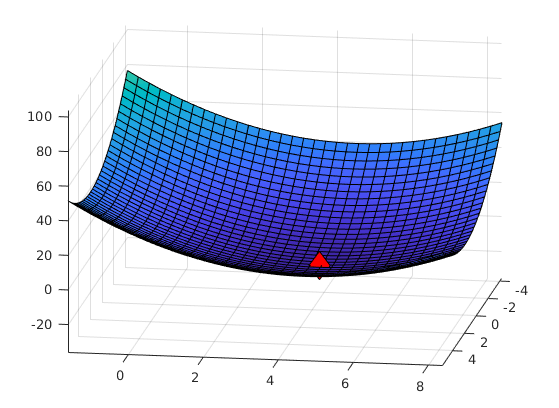
\includegraphics[scale=.4]{figs/q5.eps}
							\caption{Função custo.}
							\label{q5}
						\end{figure}
						Pode-se observar que os coeficientes de filtro ótimo, de fato, minimizam o erro quadrático médio da função ($J(\wCor)=0.15$).
			\end{enumerate}
\end{enumerate}


\bibliographystyle{ieeetr}
\bibliography{ref.bib}

\end{document}